% subseccion 4.1  
\subsection{Fase 1: Planeación}\label{sec:planeacion}
En esta etapa se estableció el propósito general para el SMS y se definieron los objetivos del estudio, preguntas de investigación, métricas, tópicos de clasificación, criterios de inclusión y exclusión y criterios de calidad. Ver Figura \ref{fig:PlanningStageOverview}.
Para los componentes ``Objetivos del estudio'', ``Preguntas de investigación'' y ``Métricas'', de la etapa de planificación, se aplicó el modelo {\itshape Goal-Question-Metric} (GQM por sus siglas en inglés) \cite{basili1992software, caldiera1994goal}. Estos componentes consideran el nivel conceptual, operacional y cuantitativo, respectivamente según \cite{Sepúlveda202141}.

\begin{figure}[htbp]
	\centering
	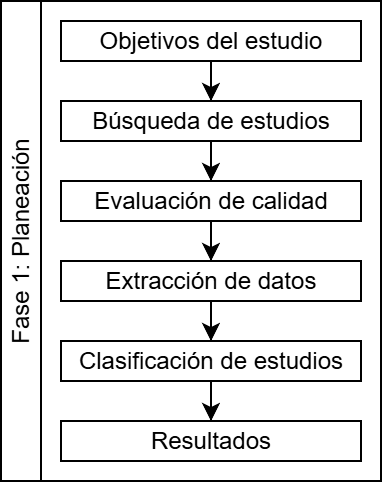
\includegraphics[scale=0.4]{resources/figures/sms-Etapa-1 overview.drawio.png}
	\caption{Componentes de la etapa de planeación.}
	\label{fig:PlanningStageOverview}
\end{figure}

% 4.1.1
%sub-subseccion - objetivos del estudio
\subsubsection{Objetivos del estudio}
Teniendo en cuenta los aspectos descritos en la sección de motivación, se han definido dos objetivos para el estudio, detallados en la Tabla \ref{table:Goals}.

\begin{table}[htbp]
	\centering
	\caption{Objetivos del SMS.}
	\label{table:Goals}
	\renewcommand{\arraystretch}{1}  % Increase row height globally
	\begin{tabular}{p{1cm}p{6.8cm}}
		\toprule
		\textbf{Objetivo} & \textbf{Descripción}                                                                                                                                                                                                                                                                                                                                         \\
		\midrule
		\textbf{G1}       & Clasificar trabajos relacionados con los universos de HTCondor según su aplicación e impacto en los dominios de computación distribuida y paralela, HTC, desarrollo de Software, virtualización y microservicios, redes de computadoras, infraestructura computacional, inteligencia artificial, análisis de datos y pensamiento computacional, entre otros. \\
		\addlinespace[0.8em]
		\textbf{G2}       & Identificar y categorizar trabajos vinculados con los universos de HTCondor como herramienta para fortalecer funciones esenciales universitarias como: investigación, docencia, extensión e industria.                                                                                                                                                       \\
		\bottomrule
	\end{tabular}
\end{table}

% 4.1.2
%sub-subseccion - pregunta de investigación
\subsubsection{Pregunta de investigación}
Para la construcción de las preguntas de investigación (RQ por sus siglas en inglés) se usó el modelo PICOC \cite{Needleman20026, Petticrew2008systematic}, que nos permite establecer los aspectos ``Población'', ``Intervención'', ``Comparación'', ``Resultados'' y ``Contexto''. Todo esto para situar el trabajo en un entorno adecuado y propender por la entrega de valor. Ver Tabla \ref{table:PICOC}.

Teniendo en cuenta la información del modelo PICOC, se definieron las preguntas de investigación (RQ por sus siglas en inglés). Ver Tabla \ref{table:RQs}.

\begin{table}[htbp]
	\centering
	\caption{Objetivos del SMS.}
	\label{table:PICOC}
	\renewcommand{\arraystretch}{1}  % Increase row height globally
	\begin{tabular}{p{1.4cm}p{6.4cm}}
		\toprule
		\textbf{Componente}   & \textbf{Descripción}                                                                                                                                                                                                                                                                                                                                                                                                                                                                             \\
		\midrule
		\textbf{Población}    & Trabajos relacionados con los universos de HTCondor según su aplicación e impacto en los dominios de computación distribuida y paralela, HTC, desarrollo de Software, virtualización y microservicios, redes de computadoras, infraestructura computacional, inteligencia artificial, análisis de datos, pensamiento computacional, entre otros. Que potencian las funciones sustantivas universitarias de investigación, docencia y extensión.                                                  \\
		\addlinespace[0.8em]
		\textbf{Intervención} & Identificación y clasificación de un conjunto de trabajos relacionados con los universos de HTCondor según su aplicación e impacto en los dominios de computación distribuida y paralela, HTC, desarrollo de Software, virtualización y microservicios, redes de computadoras, infraestructura computacional, inteligencia artificial, análisis de datos, pensamiento computacional, entre otros. Que potencian las funciones sustantivas universitarias de investigación, docencia y extensión. \\
		\addlinespace[0.8em]
		\textbf{Comparación}  & Casos de proyecto documentados; Cumplimiento de criterios de inclusión y exclusión; Aparición en bases de datos seleccionadas.                                                                                                                                                                                                                                                                                                                                                                   \\
		\addlinespace[0.8em]
		\textbf{Salidas}      & Taxonomía que organiza los trabajos relacionados con los universos de HTCondor según su aplicación e impacto en los dominios de computación distribuida y paralela, HTC, desarrollo de Software, virtualización y microservicios, redes de computadoras, infraestructura computacional, inteligencia artificial, análisis de datos, pensamiento computacional, entre otros. Que potencian las funciones sustantivas universitarias de investigación, docencia y extensión.                       \\
		\addlinespace[0.8em]
		\textbf{Contexto}     & Universos HTCondor en dominios de computación distribuida y paralela, HTC, desarrollo de Software, virtualización y microservicios, redes de computadoras, infraestructura computacional, inteligencia artificial, análisis de datos, pensamiento computacional, entre otros. Que potencian las funciones sustantivas universitarias de investigación, docencia y extensión.                                                                                                                     \\
		\bottomrule
	\end{tabular}
\end{table}

\begin{table*}[htbp]
	\centering
	\caption{Preguntas de investigación del SMS.}
	\label{table:RQs}
	\renewcommand{\arraystretch}{1}  % Increase row height globally
	\begin{tabular}{p{1cm}p{1.7cm}p{6.8cm}p{6.8cm}}
		\toprule
		\textbf{Objetivo} & \textbf{Pregunta de investigación} & \textbf{Descripción}                                                                                                                                                                                                                                                                                                                     & \textbf{Motivación}                                                                                                                                                                                                                                                                                                                                                                                    \\
		\midrule
		G1                & RQ1                                & ¿Qué trabajos relacionados con los universos de HTCondor tienen impacto en los dominios de computación distribuida y paralela, HTC, desarrollo de Software, virtualización y microservicios, redes de computadoras, infraestructura computacional, inteligencia artificial, análisis de datos y pensamiento computacional, entre otros?. & Reconocer cómo los universos de HTCondor que  tienen impacto en los dominios de computación distribuida y paralela, HTC, desarrollo de Software, virtualización y microservicios, redes de computadoras, infraestructura computacional, inteligencia artificial, análisis de datos, pensamiento computacional están estructurados, identificar sus aplicaciones y determinar su motivación contextual. \\
		\addlinespace[0.8em]
		G2                & RQ2                                & ¿Qué trabajos vinculados con los universos de HTCondor potencian las funciones esenciales universitarias como investigación, docencia, extensión e industria?.                                                                                                                                                                           & Reconocer cómo los universos de HTCondor que potencian las funciones sustantivas universitarias como investigación, docencia, extensión e industria están estructurados, identificar sus aplicaciones y determinar su motivación contextual.                                                                                                                                                           \\
		\bottomrule
	\end{tabular}
\end{table*}

% 4.1.3
%sub-subseccion - metricas
\subsubsection{Métricas}
Se definieron las métricas del SMS usando un enfoque cuantitativo de acuerdo a la estructura de clasificación. Los detalles de las métricas están en la Tabla \ref{table:Metrics}. Los criterios determinados limitan los documentos a la validez de cinco años, buscando recursos actuales en la materia. Además, el tipo de estudios fue limitado a estudios primarios, encontrados en bases de datos indexadas y reconocidas, buscando mayor rigor en la revisión por pares.

\begin{table}[htbp]
	\centering
	\caption{Métricas del SMS.}
	\label{table:Metrics}
	\renewcommand{\arraystretch}{1}  % Increase row height globally
	\begin{tabular}{p{1cm}p{6.8cm}}
		\toprule
		\textbf{Métrica} & \textbf{Descripción}                                                                                        \\
		\midrule
		\textbf{M1}      & Cantidad de trabajos seleccionados en la fase final del SMS.                                                \\
		\addlinespace[0.8em]
		\textbf{M2}      & Popularidad de cada Universo en los trabajos seleccionados en la fase final.                                \\
		\addlinespace[0.8em]
		\textbf{M3}      & Porcentaje de trabajos seleccionados en la fase final respecto a la cantidad de trabajos tenidos en cuenta. \\
		\addlinespace[0.8em]
		\textbf{M4}      & Porcentaje de trabajos seleccionados en la fase final, aportados por cada base de datos.                    \\
		\bottomrule
	\end{tabular}
\end{table}

% 4.1.4
%sub-subseccion - topicos de investigación
\subsubsection{Tópicos}
Las RQs Y el modelo PICOC sirven como la linea base para seleccionar los tópicos de clasificación usados en este trabajo. Los tópicos son los siguientes: Inteligencia artificial (AI por sus siglas en inglés), Computación en la nube, Contenerización, Computación en malla, Computación de alto rendimiento (HPC por sus siglas en inglés), Java, Virtualización, Kubernetes, Redes, Paralelismo, Docker, Computación de alta productividad (HTC por sus siglas en inglés), Educación, Investigación y Extensión.

% 4.1.5
%sub-subseccion - criterios de inclusión y exclusión
\subsubsection{Criterios de inclusión y exclusión}
Los criterios de inclusión y exclusión que se definieron para el estudio están en la Tabla \ref{table:Criteria}.

\begin{table*}[htbp]
	\centering
	\caption{Criterios de inclusión y exclusión del SMS.}
	\label{table:Criteria}
	\renewcommand{\arraystretch}{1}  % Increase row height globally
	\begin{tabular}{p{2.7cm}p{7cm}p{7cm}}
		\toprule
		\textbf{Categoría}  & \textbf{Criterios de inclusión}                                                                                                                                 & \textbf{Criterios de exclusión}                                                                                                                \\
		\midrule
		Campos              & Todos.                                                                                                                                                          & -                                                                                                                                              \\
		\addlinespace[0.8em]
		Tipo de publicación & Artículos de investigación.                                                                                                                                     & Tesis, capítulos de libros, libros, revistas, \textit{proceedings}, \textit{papers} y todo aquello no contempleado los criterios de inclusión. \\
		\addlinespace[0.8em]
		Área o disciplina   & Ciencias de la computación, Ingeniería (En la base de datos ACM se asume que todos los artículos están relacionados con estos temas ya que no permite filtrar). & Áreas no relacionadas a ciencias de la computación e ingeniería.                                                                               \\
		\addlinespace[0.8em]
		Periodo             & Desde 1980 hasta 2024.                                                                                                                                          & -                                                                                                                                              \\
		\addlinespace[0.8em]
		Idioma              & Inglés.                                                                                                                                                         & -                                                                                                                                              \\
		\bottomrule
	\end{tabular}
\end{table*}

Se definió un periodo de 44 años buscando que los estudios más relevantes en toda la historia de HTCondor sean incluidos en el mapeo de manera que (y como consecuencia de la limitada documentación encontrada en torno a esta tecnología) se haga posible para los futuros investigadores realizar una labor rigurosa tomando un periodo tan amplio y así propender por la entrega de valor del presente SMS. Adicionalmente, se limitó el tipo de estudios a artículos de revista.

\begin{equation}
	\label{equation:SCI}
	SCI = \frac{C}{A}
\end{equation}

El tercer criterio de calidad utilizado corresponde a la relación de los estudios con las preguntas de investigación; dicho criterio tiene el nombre de IRRQ (\textit{Index of Relationship to Research Questions}) (ver Formula \ref{equation:IRRQ}) donde \textit{N} corresponde a la cantidad de RQs a las cuales el estudio está relacionado. Posteriormente \textit{N} es dividido por 2 dado que esta es la cantidad de preguntas de investigación definida.

\begin{equation}
	\label{equation:IRRQ}
	IRRQ = \frac{N}{2}
\end{equation}
